\chapter{Communication Hub}
\label{ch:CPN-comm}

\section{Development Objectives}
The Single board computer (SBC) serves as the central processing node, i.e., it gathers all the data from the layers directly above and below it, then it performs the necessary computations on this data to provide control signals, feedback to electronic components, as well as feedback to the user. Thus, the SBC's development objectives can be summarized as follows:

\begin{itemize}
	\item Receive data from the web GUI to perform instructions issued by the user.
	\item Send data and logs back to the GUI to ensure proper user feedback.
	\item Receive data from the underlying micro-controllers, to utilize it in the localization process.
	\item Use all gathered data to calculate the appropriate signals and feedback that should be sent back to the micro-controllers.
\end{itemize}

To achieve the aforementioned objectives, the SBC must be capable of two types of communication, which are:
\begin{enumerate}
	\item Upwards communication: which is the type of communication concerned with receiving user input and providing feedback.
	\item Downwards communication: which is the the type of communication that is concerned with receiving sensors' readings from micro-controllers and issuing commands to execute the assigned tasks.
\end{enumerate}

In the subsequent sections we discuss the implementation of these objectives at greater length.

%\section{First Objective: Communication Hub}
% I want to remove the "First objective" part
% Sure thing, fam
\section{Proposed Communication Model} % + state reason behind using them
Different tools are used to accomplish the two desired types of communication: Upward and Downward Communication; both will be explained in the following subsections.
\newpage
\subsection{Upwards Communication}
There are two types of data that the SBC needs to receive from the server. The first type of data is the direct user request, this is what the SBC receives when the user requests that the robot moves with a specific speed, or when the user starts a given task. In short, the request data type is directly triggered by a user action.

Requests are sent from the server to the SBC using the Axios framework, which will be discussed in further detail in the next chapter, but in short, it is a tool used to send requests from the front-end of a web application to some endpoint. Axios uses XML and HTTP to accomplish this goal \cite{axios-intro}. These requests are sent from the user-facing GUI to the PHP back-end that is running on the SBC.

The other data type that the SBC needs to receive from the server is files. Some user input is too complex to encapsulate in a single request, so these inputs are collected in files on the server, which are then sent to the SBC. The two main types of files are map files and task files, both of which are of the commonly used JavaScript Object Notation (JSON) format. Map json files contain details about the maps that the user creates in the GUI. For example it contains the identifiers and labels of every node in the map, the relation between nodes (which nodes are connected with wich nodes), and the absolute position of every node. A simple map json file is shown in code snippets \ref{cd:sampleMap} and \ref{cd:sampleMap2}.

\lstinputlisting[style=CodeStyleJSON, caption=Sample JSONn Map File, label=cd:sampleMap, firstline=1, lastline=20]{./CodeSnippets/sample-map.json}

\newpage

\lstinputlisting[style=CodeStyleJSON, caption=Sample JSONn Map File (Continued), label=cd:sampleMap2, firstline=21, lastline=52]{./CodeSnippets/sample-map.json}

\newpage

Similarly, when the user creates a new task to be executed by a robot, this task is saved to a json file on the server. A sample task file is shown in code snippet \ref{cd:sampleTask}.

\lstinputlisting[style=CodeStyleJSON, caption=Sample json task file, label=cd:sampleTask]{./CodeSnippets/sample-task.json}

The shown files are created on the server and need to be synchronized with the SBC. The desired feature is synchronization and not simple file transfer because these files represent maps and tasks that the user may edit or delete, so it is desirable to have these changes synchronized between the server and the SBC.

The tool that is used to accomplish this synchronization is RSYNC, which is a fast file synchronization tool for both remote and local files \cite{rsync-github}. The bash script shown in code snippet \ref{cd:rsync} is used to synchronize the maps and tasks directories between the server and the SBC.

The script uses the server's IP address to communicate with the server. The SBC has a number of ssh keys used for authentication, one of which is used by RSYNC for authentication between the SBC and the server. But for this to work properly, the ssh-agent must be running on the SBC to enable automatic authentication. Lastly RSYNC is used to synchronize its target directories, i.e., the maps directory on the server and its corresponding directory on the SBC, and the same is true for the tasks directory.

The system administrator is free to change:
\begin{itemize}
	\item IP address of the server.
	\item Which ssh keys are used for authentication (in script \ref{cd:rsync} all available ssh keys are added for good measure).
	\item The directories that RSYNC targets for synchronization.
\end{itemize}

\newpage

\lstinputlisting[language=Bash, style=CodeStyleBash, caption=Synchronization script, label=cd:rsync]{./CodeSnippets/sync-maps-tasks.sh}

Another form of upwards communication is the feedback that the SBC provides for the user, the main type of this feedback is the camera stream. The robot is equipped with a stereo camera, this camera's stream is then broadcast on the network for the user to view.
The camera is shown in figure \ref{fig:stereo-cam}, this stereo camera is connected to the SBC using USB. The stream from this camera is broadcast on the network using a the mjpg-streamer, which is a command line application that copies JPEG frames from one or more input plugins to multiple output plugins\cite{mjpg-streamer}. In this specific instance, the input plugin that is used is the input\_uvc.so plugin, which deals with USB input cameras, and the output plugin is the output\_http.so plugin, which allows mjpg-streamer to broadcast the stream using HTTP.
\begin{figure}[h!]
	\centering
	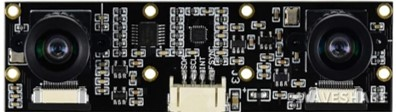
\includegraphics[scale=0.8]{./Figures/cam.jpg}
	\caption{Stereo camera}
	\label{fig:stereo-cam}
\end{figure}

\subsection{Downwards Communication}
Downwards communication is mainly accomplished using the Robot Operating System (ROS) which is a set of software libraries and tools that are used to build robot applications\cite{ros_documentation}. 
\newpage
When building an application using ROS, the application logic is broken into a number of ROS nodes, where these nodes communicate using ROS topics. When a node produces data it is then called a publisher, that is because this data is published on a specific topic. When a node receives data it is then called a subscriber, that is because it subscribes to the appropriate ROS topic that contains the data of interest. This data is called ROS messages, and each ROS topic supports a specific type of messages. For example, some ROS topics support only integer data, so all nodes publishing on this topic must only publish integer data, and all nodes subscribing to this topic must only expect to receive integer data. Figure \ref{fig:ros_arch_official} shows the relation between the different ROS nodes on the system as well as the ROS topics\cite{ros_documentation}. There have been many ROS releases over the years, here we use ROS Noetic, which is primarily targeted for machines that run Ubuntu 20.04 LTS as their operating system. In other words, newer versions of Ubuntu will not be compatible with ROS Noetic.
\begin{figure}[h!]
	\centering
	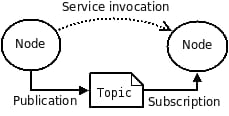
\includegraphics[scale=0.8]{./Figures/CentralProcessingNode/UsedToolsAndFrameworks/Ros-images/ros-arch-official.jpeg}
	\caption{Communication Between ROS Nodes}
	\label{fig:ros_arch_official}
\end{figure}


We will define some of the basic concepts needed to understand ROS and how to use it:
\begin{itemize}
	\item Packages: 
	
	They are the primary unit for organizing software in ROS. They can contain ROS runtime processes (nodes), ROS-dependent libraries, datasets, configuration files, or any other related components. In ROS, packages are the smallest units of build and release, meaning that the smallest entity you can build and release is a package.
	\item Package Manifests
	
	Package manifests (package.xml) provide metadata about a package, including its name, version, description, license information, dependencies, and other metadata such as exported packages.
	
	\item Message (msg) Types:
	
	Message types, define the data structures for messages sent within ROS.

	There are several types of messages used to facilitate communication between nodes. These message types are defined by their content and structure. The main types of ROS messages are:
		\newpage
	\begin{enumerate}
		\item Standard Messages:
		
		These are the predefined message types provided by ROS. They cover a wide range of common data structures and are grouped into different categories:
		
		\begin{itemize}
			\item std\_msgs: 
			Contains simple message types like Bool, Int32, Float64, String, etc.
			\item geometry\_msgs:
			Includes messages for geometric primitives like Point, Vector3, Pose, Twist, etc.
			\item sensor\_msgs:
			Contains messages related to sensor data like Image, Imu, LaserScan, NavSatFix, etc.
		\end{itemize}
		\item Custom Messages:
		
		Users can define their own message types to suit their specific application needs. Custom messages are defined in .msg files within a ROS package and can include various data types such as integers, floats, strings, arrays, and other message types.
	\end{enumerate}  
	  
	\item Nodes:
	
	Nodes are processes that perform computations. ROS is designed for fine-grained modularity, meaning a robot control system typically comprises many nodes. For example, one node might control a laser range-finder, another controls the wheel motors, another handles localization, another performs path planning, and yet another provides a graphical view of the system. Nodes in ROS are written using a ROS client library such as roscpp or rospy.
	
	\item Master: 
	
	The ROS Master provides name registration and lookup services for the Computation Graph. Without the Master, nodes would be unable to locate each other, exchange messages, or invoke services.
	% \newpage
	\item Topics:
	
	Messages are routed via a transport system using publish/subscribe semantics. A node sends a message by publishing it to a specific topic, a name identifying the message content. Nodes interested in certain data subscribe to the appropriate topic. Multiple publishers and subscribers can exist for a single topic, and a single node can publish and/or subscribe to multiple topics. Publishers and subscribers are generally unaware of each other's existence, which decouples information production from its consumption. Logically, a topic functions as a strongly typed message bus, with each bus having a name. Anyone can connect to the bus to send or receive messages, provided they use the correct type.
\end{itemize}



% \subsection{Communication protocols for the Proposed Design}

% \subsection{Output} % + state which of the listed specs were fulfilled here

%%%%%%%%%%%%%%%%%%%%%%%%%%%%%%%%%%%%%%%%%%%%%%%%%%%%%%%%%%%%%%%%%%%%%%%%%%%%%%%%%




%%%%%%%%%%%%%%%%%%%%%%%%%%%%%%%%%%%%%%%%%%%%%%%%%%%%%%%%%%%%%%%%%%%%%%%%%%%
\newpage
\chapter{Indoor Localization}
\label{ch:loc}
\section{Development Objectives}
Through the robot runtime, it will receive missions in which cargo shall be transmitted from one place to another. Each place has its own set of information, which can either be related to the place itself, related to adjacent places, or assigned by the infrastructure. In light of all of this, the robot should be able to:
\begin{itemize}
	\item Determine the best path from current location to target destination.
	\item Localize itself using existing infrastructure.
	\item Integrate various sensor inputs to maintain accurate localization.
\end{itemize}

\section{Methods of Localization}
Through investigating different means of localization, an approach involving Dead Reckoning technique for position estimation accompanied with an Extended Kalman Filter (EKF) to improve estimation performance was selected. The output of Dead Reckoning algorithm will be processed by the EKF in addition to IMU data in order to provide precise position estimation. This method is labeled Odometry Localization for the rest of the chapter.

Additionally, Visible Light Communication (VLC) is used as an auxiliary means of localization; offering several advantages over other methods such as Radio Frequency (RF) localization:

\begin{itemize}
	\item It uses the unlicensed visible light portion of the spectrum.
	\item It makes use of the existing LEDs in the facility for both illumination and data transmission, while consuming less power than other RF transmitters.
	\item It depends on the inherent need of Line-Of-Sight (LOS) and the inability to penetrate through walls, making it more secure.
\end{itemize}

\newpage

Localization via VLC can be classified into two categories depending on the specific implementation details and use cases, which are: \textbf{Direct Positioning}; where the receiver uses all received information (i.e. time of arrival, angle of arrival) from transmitters to directly determine its position, and \textbf{Two-Step Positioning}, in which the receiver first extracts position-related parameters from the transmitter, then processes these parameters using algorithms to determine its location. 
For its convenience, the two-step positioning approach is utilized, and more specifically the \textbf{proximity method}.% \cite{vlp} 

\subsection{Odometry}
The localization system uses a combination of dead reckoning and sensor fusion to maintain an accurate estimate of the robot's position. The dead reckoning algorithm is implemented in the \textbf{dead\_reckoning.py} script, which updates the robot's position based on wheel encoder data and publishes it as an odometry ROS message.

\subsubsection{Forward Kinematics}
Forward kinematics involves calculating the position and orientation of the robot based on the joint parameters (e.g., wheel rotations). The dead reckoning script shown in code snippet \ref{cd:dead-reckoning} in Appendix D includes the implementation of forward kinematics for a differential drive robot.


The script calculates the changes in position ($\Delta x$, $\Delta y$) and orientation ($\Delta \theta$) based on the velocity commands received and updates the robot's position accordingly.

\subsubsection{Inverse Kinematics}
Inverse kinematics involves calculating the joint parameters needed to achieve a specific position and orientation of the robot. In the context of a differential drive robot, inverse kinematics can be derived from the desired linear and angular velocities to determine the individual wheel speeds. The implementation is shown in code snippet \ref{cd:inverse-kinematics} located in Appendix D.


\subsubsection{Sensor Fusion using EKF}
The EKF is configured to combine odometry data and IMU data to provide a more accurate and robust localization estimate. The EKF configuration is provided in code snippet \ref{cd:efk-launch} situated in Appendix D.

\newpage

\subsection{Visible Light Communication:}
In the proximity method, each transmitter (i.e. LED) continuously sends a code specific to its location. As the robot moves, the receiver receives information from the closest transmitter, then uses algorithms to determine the code, thus knows its location. This method is chosen as a trade-off between its simplicity and its inaccuracy in localization. However, the used applications for the robot may not require much accuracy.
\cite{vlp} \cite{indoor-vlp}

\begin{figure}[h!]
	\centering
	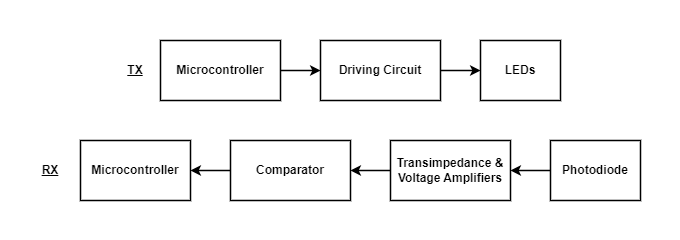
\includegraphics[scale=0.5]{Figures/HW/VLC-blk.png}
	\caption{The Block Diagram for The Used VLC system}
	\label{fig:hw-vlc-blk}
\end{figure}

The structure of the used VLC system is shown in figure \ref{fig:hw-vlc-blk}. The code is assigned to every location and stored in a micro-controller, which periodically drives some LEDs. The signal transmitted by the LEDs are then received through a photodiode. The received signal is then amplified, then passes through a comparator to produce 0's and 1's, to be finally received by another microcontroller responsible for storing the received code, processing it and determining its location based on it.

\begin{figure}[h!]
	\centering
	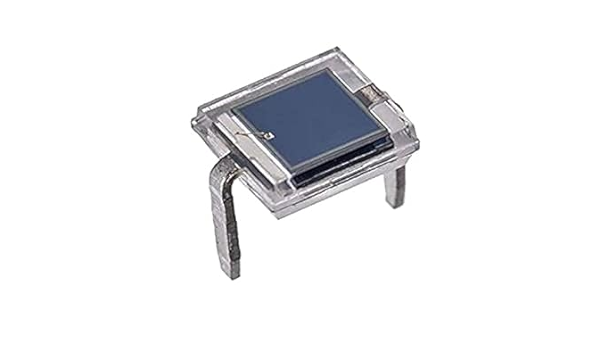
\includegraphics[scale=0.4]{Figures/HW/BPW34.png}
	\caption{BPW34 Photodiode}
	\label{fig:hw-vlc-pd}
\end{figure}


The key element of the receiver system is the \textbf{photodiode}, in this case, a BPW34 shown in figure \ref{fig:hw-vlc-pd}, which designed to work within wavelengths \textbf{[420:1100] nm}, produce open-circuit voltage up to \textbf{350 mV}, and short circuit current up to \textbf{70 $\mu$A }. It acts just like a solar-cell: when light falls on it, it generates current to its load. \cite{BPW34-datasheet}.

\newpage

The issue is dealing with the BPW34 directly is quite difficult; since its current is in the $\mu$A. A solution this problem is to convert this insignificant current into more measurable voltage through a \textbf{Transimpedance Amplifier} (or TI). It is designed to amplify the light-dependent current of the photodiode. 

\begin{figure}[h!]
	\centering
	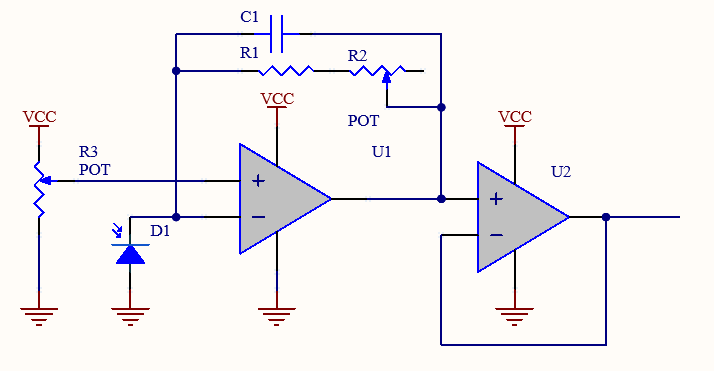
\includegraphics[scale=0.5]{Figures/HW/ti-amp-buffer.png}
	\caption{The Transimpedance Amplifier Stage of The Implemented Receiver}
	\label{fig:hw-ti-buffer}
\end{figure}


In the actual receiver shown in figure \ref{fig:hw-ti-buffer} the TI amplifier is designed to to be modified based on the transmitter and surrounding conditions, by modifying $R_2$, and the potentiometer $R_3$ controls its offset. The output of the TI is followed by a buffer to provide a low impedance output for the next stage. \cite{op-amp-circuits} 

The output voltage the first stage has a range of about \textbf{0.7 V}, which may not be difficult to process. It is desired to: 
\begin{itemize}
	\item Increase the output voltages.
	\item Increase the voltage range, allowing for more accurate decision making. 
\end{itemize}
Both of these objectives can be achieved by following the first stage with a non-inverting amplifier. A voltage gain ratio of 2 should be enough.

The final stage for the receiver is the decision making. Ideally, a comparator circuit with one threshold would work well, however, it comes with some issues:
\begin{itemize}
	\item Unstable output when the input is very close to the threshold.
	\item The value for a '0' or a '1' can fluctuate causing misreadings in the middle of a single bit.
\end{itemize}

One way to optimize this behaviour is using a Schmitt Trigger for decision makinhg, which is basically a comparator with an upper and lower thresholds, where if and only if:
\begin{itemize}
	\item $V_{in} > V_u$, $V_{out}$ is HIGH. 
	\item $V_{in} < V_l$, $V_{out}$ is LOW. 
\end{itemize}
Where $V_u$ and $V_l$ are the Schmitt Trigger upper and lower thresholds respectively.

\newpage

\begin{figure}[h!]
	\centering
	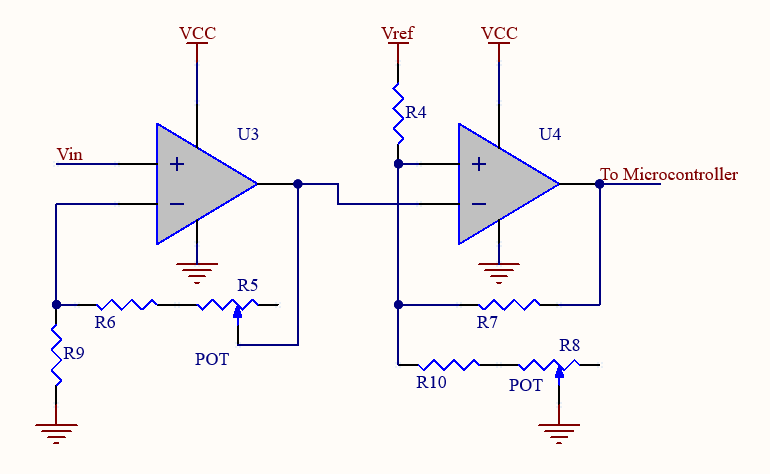
\includegraphics[scale=0.45]{Figures/HW/amp-schmitt.png}
	\caption{The second stage of the receiver: Non-inverting Amplifier (Left) and inverting Schmitt Trigger (Right)}
	\label{fig:hw-amp-schmitt}
\end{figure}

The used schmitt trigger in the actual circuit is an inverting one, so $V_{out}$ inverted from what was mentioned above. To design the second stage with proper components, LTSpice was used for simulation, as found in figure \ref{fig:hw-amp-schmitt-sim}. The results can be found on figure \ref{fig:hw-amp-schmitt-results}. It noted that $V_{amplified}$ is clamped from the negative side due to the presence of ground instead on negative voltage. On the other hand, to prevent clamping on the positive side for the amplifier, the 12V supply can be used to power it.

\begin{figure}[h!]
	\centering
	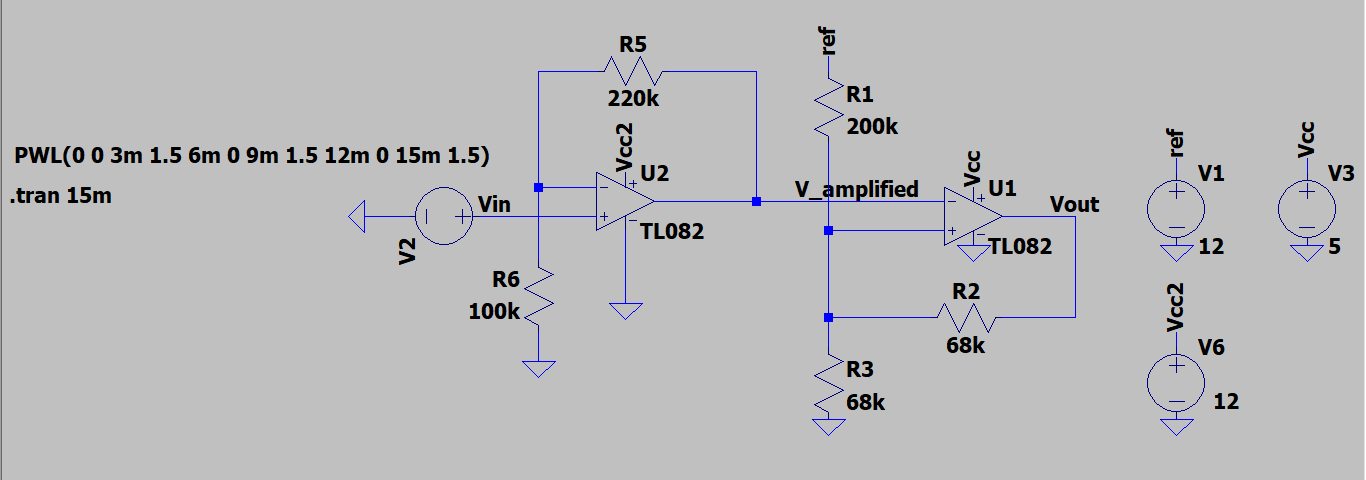
\includegraphics[scale=0.35]{Figures/HW/amp-schmitt-ltspice.png}
	\caption{Simulating The second phase of the receiver on LTSpice.}
	\label{fig:hw-amp-schmitt-sim}
\end{figure}

\begin{figure}[h!]
	\centering
	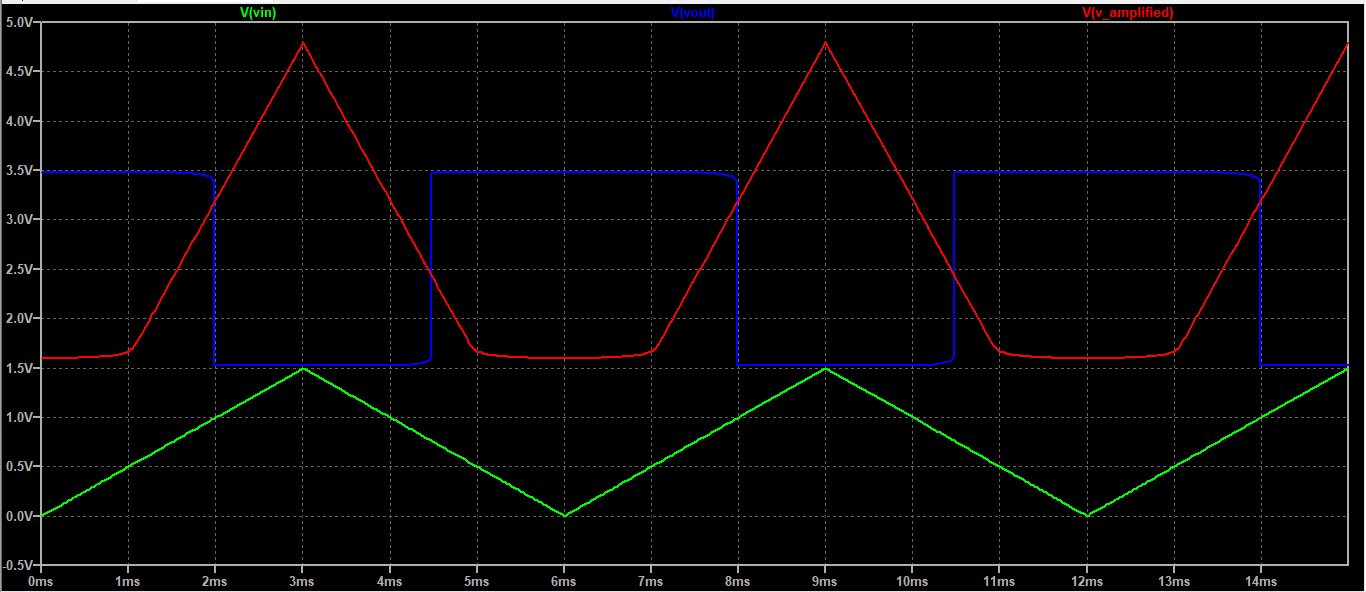
\includegraphics[scale=0.35]{Figures/HW/amp-schmitt-ltspice-results.png}
	\caption{The results of simulation.}
	\label{fig:hw-amp-schmitt-results}
\end{figure}

% Kid, I don't have much time

% The secret of DIO's stand is sto
% :""""
% DIO! Yaro!
%\newpage
%\section{Output}
%The localization system meets the following specifications:
%\begin{itemize}
%	\item Accurate path determination from current location to target location.
%	\item Real-time localization using existing infrastructure and sensor fusion.
%	\item Robust integration of various sensor inputs to maintain accuracy.
%\end{itemize}



%The EKF setup integrates multiple sensor inputs to enhance the accuracy of the robot's localization.